En este capítulo se describen los procesos de operación relacionados a los módulos hechos durante este trabajo terminal. \\

Se definieron los roles que se encargan de registrar la informacón por módulo así como el proceso general operativo. Los roles definidos son los siguientes:

\begin{itemize}
	\item {Encargado de registro de infraestructura}
	\item {Encargado de registro de unidades de aprendizaje}
	\item {Encargado de registro de profesores}
	\item {Encargado de registro de convocatorias de movilidad}
	\item {Encargado de registro de convocatorias de cursos}
\end{itemize}

\subsection{Proceso Operativo}

En la figura \ref{fig:macro} se muestra el macroproceso en donde intervienen los cinco encargados de los diferentes módulos, así como la interacción del alumno en los mismos. \\
De acuerdo al flujo mostrado en la figura \ref{fig:macro} se pueden tomar los siguientes cursos de acción:  

\begin{itemize}
	\item {Se puede realizar la gestión de los espacios y la gestión de convocatorias de movilidad sin necesidad de contar con información previa y terminar con el proceso.}
	\item {Posterior a la carga de información en el módulo de salones se puede pasar a la gestión de unidades de aprendizaje y a la gestión de cursos.}
	\item {Ya que se cuenta con información de espacios y de unidades de aprendizaje se puede gestionar profesores, dado que en el módulo se requiere información registrada en los módulos antes mencionados.}
\end{itemize}

\begin{figure}[h!]
	\begin{center}
		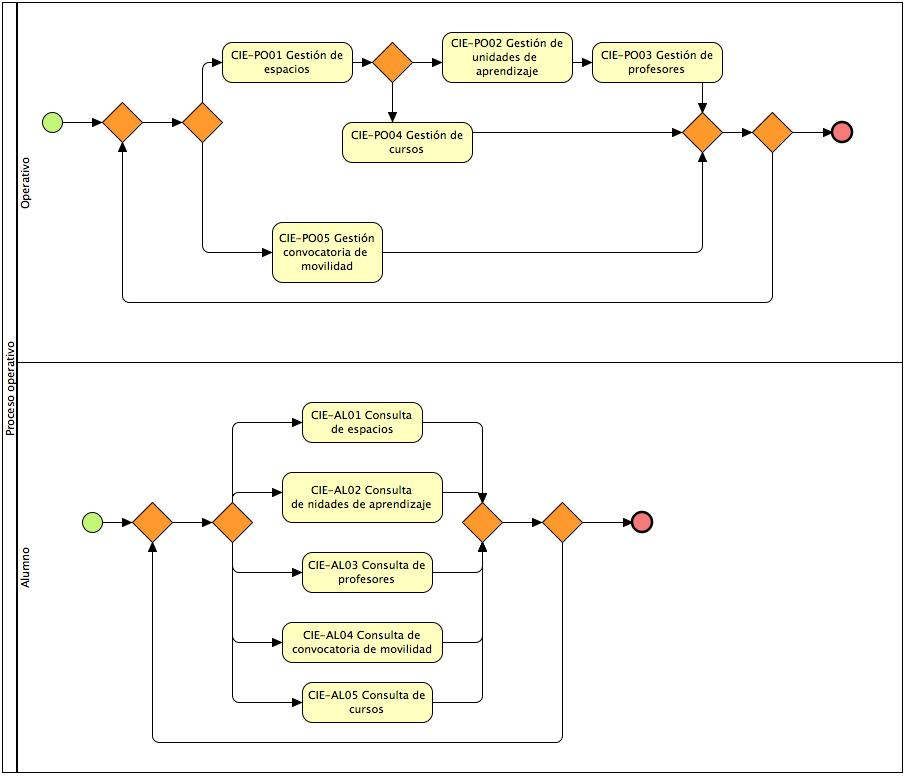
\includegraphics[width=1\textwidth]{images/procesos/macro.jpg}
		\caption{Proceso operativo.}
		\label{fig:macro}
	\end{center}
\end{figure}

En la parte baja del diagrama podemos ver el proceso del alumno para la consulta de información en los diversos módulos de la aplicación. El alumno puede seguir el flujo del diagrama en cualquier dirección y no cuenta con restricciones de consulta entre un módulo y otro.

\subsection{Proceso del encargado de registro de infraestructura.}

En la figura \ref{fig:espacios} se muestra el diagrama del proceso para el encargado de registro de infraestructura. El flujo comienza desde el lado izquiero y continúa a la derecha. \\

En el flujo del proceso se muestra la siguiente condición:
Para poder registrar un nuevo salón, debe existir al menos un edificio registrado, con niveles y detalle del mismo de manera que el nuevo salón pertenezca a tal edificio. \\

El encargado puede registra un nuevo edificio, registrar el detalle del nuevo edificio, registrar los niveles del edificio, registrar salones, así como editar edificios y salones y eliminar los salones.

\begin{figure}[h!]
	\begin{center}
		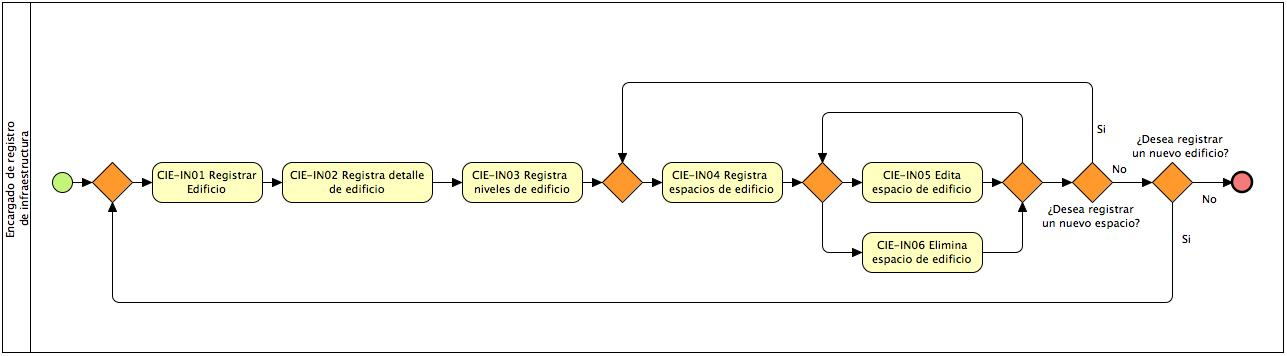
\includegraphics[width=1\textwidth]{images/procesos/espacios.jpg}
		\caption{Proceso del encargado de registro de infraestructura.}
		\label{fig:espacios}
	\end{center}
\end{figure}

\subsection{Proceso del encargado de registro de unidades de aprendizaje.}

La figuta \ref{fig:unidades} muestra el proceso para el encargado de registro de unidades de aprendizaje. En la figura se puede observar el flujo para registrar una unidad de aprendizaje, de la misma manera para editar y eliminar la misma. \\

Para lograr hacer un regisrro exitoso es necesario primero contar con el programa académico de la unidad de aprendizaje. 

\begin{figure}[h!]
	\begin{center}
		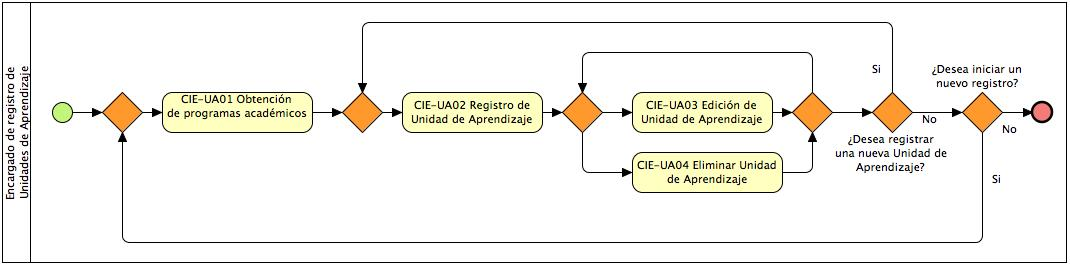
\includegraphics[width=1\textwidth]{images/procesos/unidades.jpg}
		\caption{Proceso del encargado de registro de unidades de aprendizaje.}
		\label{fig:unidades}
	\end{center}
\end{figure}

\subsection{Proceso del encargado de registro de profesores.}

En la figura \ref{fig:profesores} se muestra el proceso para el encargado de registro de los profesores. Es importante mencionar que antes de obtener información ya sea pública o personal, el encargado debe elaborar un aviso de privacidad y debe obtener el consentimiento de los profesores antes de publicar su información. \\

Después de obtener la información, el encargado puede registrar, editar y eliminar a un profesor así como obtener nuevas firmas de profesores que ingresen posteriormente y mantener una base de datos completa del personal docente.

\begin{figure}[h!]
	\begin{center}
		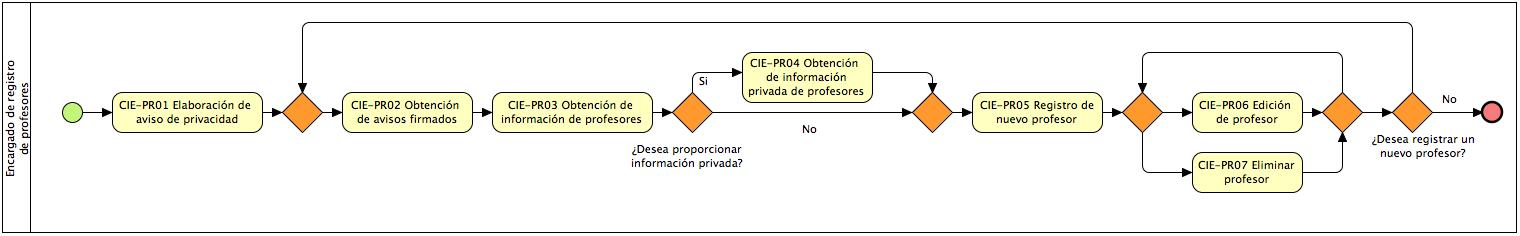
\includegraphics[width=1\textwidth]{images/procesos/profesores.jpg}
		\caption{Proceso del encargado de registro de profesores.}
		\label{fig:profesores}
	\end{center}
\end{figure}

\subsection{Proceso del encargado de registro de convocatorias de movilidad.}

En la figura \ref{fig:movilidad} se muestra el proceso para el encargado de registro de convocatorias de movilidad. \\

El flujo que muestra el proceso nos indica que el encargado, antes de ponder publicar los enlaces a la convocatoria actual de movilidad, de revisar qu el Instituto haya publicado una nueva. Con base en lo anterior, el encargado de registro puede publicar tanto la convocatoria como las universidades participantes tanto en su modalidad de movilidad nacional como internacional. Posterior a la publicación de convocatoria y universidades, el encargado debe obtener los resultados de acuerdo a la fecha prevista por el Instituo y publicarlos así en el módulo correspondiente.

\begin{figure}[h!]
	\begin{center}
		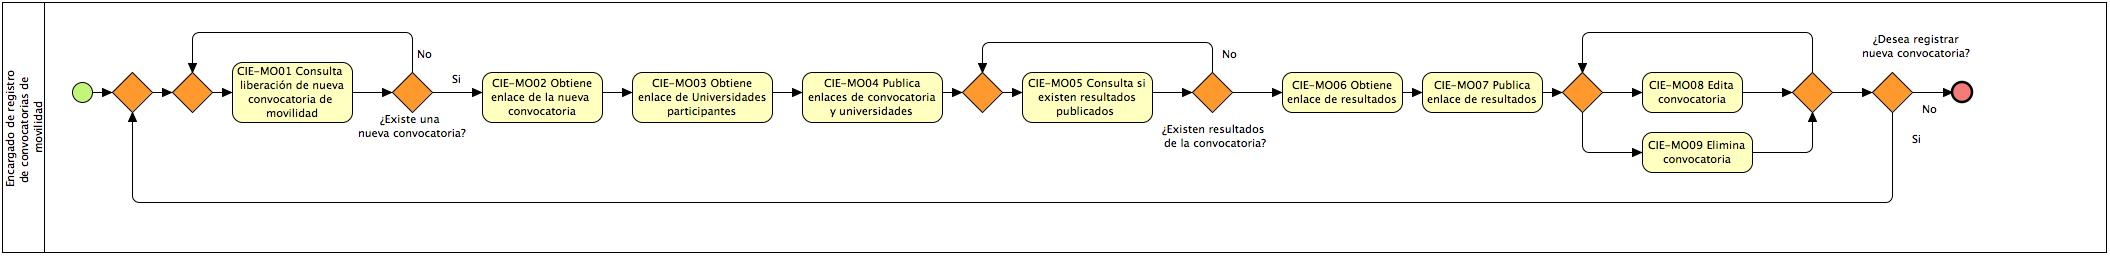
\includegraphics[width=1\textwidth]{images/procesos/movilidad.jpg}
		\caption{Proceso del encargado de registro de convocatorias de movilidad.}
		\label{fig:movilidad}
	\end{center}
\end{figure}

\subsection{Proceso del encargado de registro de convocatorias de cursos.}

En la figura \ref{fig:cursos} se muestra el proceso para el encargado de registro de convocatorias para cursos. \\

Siguiendo el flujo del proceso, el encargo de registro debe obtener la información del curso por parte de la persona que lo esté gestionando. Tomando como ejemplo la Escuela Superior de Cómputo, centros de investigación como el CIC o el CIDETEC suelen ofrecer también cursos relacionados con el programa académico de la ESCOM, por lo tanto pueden ser recibidos y publicados para la comunidad de la escuela. \\

Además de registrar nuevos cursos, el encargado de registro de convocatorias de cursos puede editar una convocatoria existente y eliminarla.

\begin{figure}[h!]
	\begin{center}
		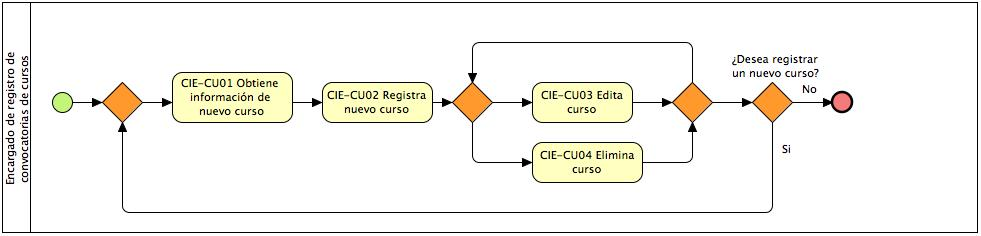
\includegraphics[width=1\textwidth]{images/procesos/cursos.jpg}
		\caption{Proceso del encargado de registro de convocatorias de cursos.}
		\label{fig:cursos}
	\end{center}
\end{figure}